\documentclass[a4paper]{article}
\usepackage[pdftex]{hyperref}
\usepackage[latin1]{inputenc}
\usepackage[english]{babel}
\usepackage{a4wide}
\usepackage{amsmath}
\usepackage{amssymb}
\usepackage{algorithmic}
\usepackage{algorithm}
\usepackage{ifthen}
\usepackage{listings}
\usepackage{array}
\usepackage{tabu}
% move the asterisk at the right position
\lstset{basicstyle=\ttfamily,tabsize=4,literate={*}{${}^*{}$}1}
%\lstset{language=C,basicstyle=\ttfamily}
\usepackage{moreverb}
\usepackage{palatino}
\usepackage{multicol}
\usepackage{tabularx}
\usepackage{comment}
\usepackage{verbatim}
\usepackage{color}
\usepackage{graphicx}
\usepackage{array,mathtools}
\usepackage{amsmath}
\usepackage{enumitem,amssymb}
\usepackage{pifont}
\newlist{todolist}{itemize}{2}
\setlist[todolist]{label=$\square$}
\newcommand{\cmark}{\ding{51}}%
\newcommand{\xmark}{\ding{55}}%
\newcommand{\done}{\rlap{$\square$}{\raisebox{2pt}{\large\hspace{1pt}\cmark}}%
\hspace{-2.5pt}}
\newcommand{\wontfix}{\rlap{$\square$}{\large\hspace{1pt}\xmark}}



%% pdflatex?
\newif\ifpdf
\ifx\pdfoutput\undefined
\pdffalse % we are not running PDFLaTeX
\else
\pdfoutput=1 % we are running PDFLaTeX
\pdftrue
\fi
\ifpdf
\fi
\ifpdf
\DeclareGraphicsExtensions{.pdf, .jpg}
\else
\DeclareGraphicsExtensions{.eps, .jpg}
\fi

\parindent=0cm
\parskip=0cm

\setlength{\columnseprule}{0.4pt}
\addtolength{\columnsep}{2pt}

\addtolength{\textheight}{5.5cm}
\addtolength{\topmargin}{-26mm}
\pagestyle{empty}

%%
%% Sheet setup
%% 
\newcommand{\coursename}{Computer Architecture and Programming Languages}
\newcommand{\courseno}{CO20-320241}
\newcommand*{\carry}[1][1]{\overset{#1}}
\newcolumntype{B}[1]{r*{#1}{@{\,}r}}
 
\newcommand{\sheettitle}{Homework}
\newcommand{\mytitle}{}
\newcommand{\mytoday}{{2nd of December}, 2019}

% Current Assignment number
\newcounter{assignmentno}
\setcounter{assignmentno}{11}

% Current Problem number, should always start at 1
\newcounter{problemno}
\setcounter{problemno}{1}

%%
%% problem and bonus environment
%%
\newcounter{probcalc}
\newcommand{\problem}[2]{
  \pagebreak[2]
  \setcounter{probcalc}{#2}
  ~\\
  {\large \textbf{Problem \textcolor{blue}{\arabic{assignmentno}}.\textcolor{blue}{\arabic{problemno}}} \hspace{0.2cm}\textit{#1}} \refstepcounter{problemno}\vspace{2pt}\\}

\newcommand{\bonus}[2]{
  \pagebreak[2]
  \setcounter{probcalc}{#2}
  ~\\
  {\large \textbf{Bonus Problem \textcolor{blue}{\arabic{assignmentno}}.\textcolor{blue}{\arabic{problemno}}} \hspace{0.2cm}\textit{#1}} \refstepcounter{problemno}\vspace{2pt}\\}

%% some counters  
\newcommand{\assignment}{\arabic{assignmentno}}

%% solution  
\newcommand{\solution}{\pagebreak[2]{\bf Solution:}\\}

%% Hyperref Setup
\hypersetup{pdftitle={Homework \assignment},
  pdfsubject={\coursename},
  pdfauthor={},
  pdfcreator={},
  pdfkeywords={Computer Architecture and Programming Languages},
  %  pdfpagemode={FullScreen},
  %colorlinks=true,
  %bookmarks=true,
  %hyperindex=true,
  bookmarksopen=false,
  bookmarksnumbered=true,
  breaklinks=true,
  %urlcolor=darkblue
  urlbordercolor={0 0 0.7}
}

\begin{document}


\coursename \hfill Course: \courseno\\
Jacobs University Bremen \hfill \mytoday\\
Fjolla Dedaj\hfill
\vspace*{0.3cm}\\
\begin{center}
{\Large \sheettitle{} \textcolor{blue}{\assignment}\\}
\end{center}
\problem{}{0}
Use the data from the example given on slide $29 ($Lecture $20 $ \& $ 21)$ and assume that you have to execute a program containing 2 load instructions, 1 store instruction, 3 R-format instructions and 1 branching instruction for computing the speedup relate to the execution time in the following scenarios:\\
\\
(a) multi-cycle approach compared to single cycle approach, \\
(b) pipelined approach compared to single cycle approach, \\
(c) pipelined approach compared to multi-cycle approach.\\
\\
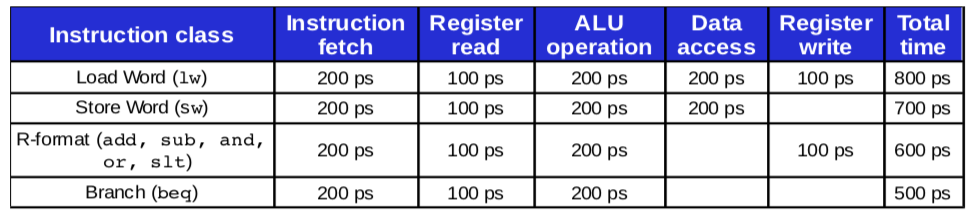
\includegraphics[scale=0.45]{skrin1.png}
\\
\\
\solution
\textbf{Single Cycle Approach:}\\
Find the instruction that takes the longest to complete and multiply that with the total number of instructions because each instruction will take the same amount of time. Thus, we have:\\
\\
$(2 + 1 + 3 + 1) \times 800 = 7 \times 800 = 5600$\\
\\
\textbf{Multi-Cycle Approach:}\\
Each instruction will take its respective amount of time to complete. Therefore, we have:\\
\\
$2 \times 800 + 1 \times 700 + 3 \times 600 + 1 \times 500 = 4600$\\
\\
\textbf{Pipelined Approach:}\\
The instructions happen concurrently, however, we have a delay for the instruction fetch:\\
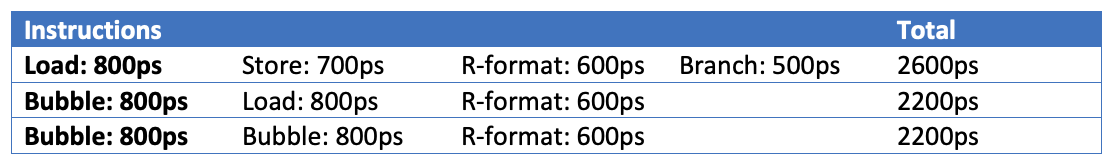
\includegraphics[scale=0.4]{skrin2.png}\\
The processing stage taking the longest is: 2600ps\\
\\
Calculate the time rates:\\
\\
\textbf{(a)} $\frac{single-cycle}{multi-cycle} = \frac{5600}{4600} = 1.2173913$\\
\\
\textbf{(a)} $\frac{single-cycle}{pipelined} = \frac{5600}{2600} = 2.15384615$\\
\\
\textbf{(a)} $\frac{multi-cycle}{pipelined} = \frac{4600}{2600} = 1.76923077$\\
\\
\pagebreak
\\
\problem{}{0}
\solution
(a) the string \$zero:\\
\textbf{\$zero}\\
\\
(b) all strings which start with a and end with b and may contain any other letters or digits:\\
\textbf{\textbackslash{a}[a-zA-Z0-9]*\textbackslash{b}}\\
\\
(c) all strings which start and end with a digit and may contain letters, digits, and underscores:\\
\textbf{[0-9][a-zA-Z0-9\_]*[0-9]}\\
\\
(d) all strings which contain only the characters a and b, start with abb following by at least 4
a, the total length of the string should not be longer than 10 characters:\\
\textbf{"abb"a\{4\}[ab]\{0,3\}}\\
\\
(e) all positive integer numbers:\\
\textbf{[1-9]+[0-9]*}\\
\\
(f) all integer numbers:\\
\textbf{[-]?[1-9]+[0-9]*}\\
\\
(g) all positive floating point numbers:\\
\textbf{[0-9]*[.]?[0-9]*}\\
\\
(h) the strings pit, spot, spate, slap two, respite but it should not recognize the strings pt, Pot, peat, part:\\
\textbf{$(\text{pit}|\text{spot}|\text{spate}|\text{slap two}|\text{respite})$}\\
\problem{}{0}
\solution
Correct answers are denoted in bold.\\
\\
(a) ab+c? (including ?)\\
\\
\textbf{(1) abc}\\
(2) ac\\
\textbf{(3) abbb}\\
(4) bbc\\
\\
(b) a.[bc]+\\
\\
\textbf{(1) abc}\\
\textbf{(2) abbbbbbbb}\\
\textbf{(3) azc}\\
\textbf{(4) abcbcbcbc}\\
(5) ac\\
\textbf{(6) asccbbbbcbcccc}\\
\\
(c) (very )+(happy )?((CS)|(IMS)|(ECE)) student\\
\\
(1) very happy student\\
(2) happy CS student\\
\textbf{(3) very very happy ECE student}\\
\textbf{(4) very very very happy IMS student}\\
\textbf{(5) very very very very IMS student}\\
\\
(d) $<[ \, \wedge > ] \, $ $+>$\\
\\
\textbf{(1) $<$an xml tag$>$}\\
\textbf{(2) $<$opentag$>$ $<$closetag$>$}\\
\textbf{(3) $<$/closetag$>$}\\
(4) $<>$\\
\textbf{(5) $<$with attribute $>$}
\end{document}